\begin{figure}
    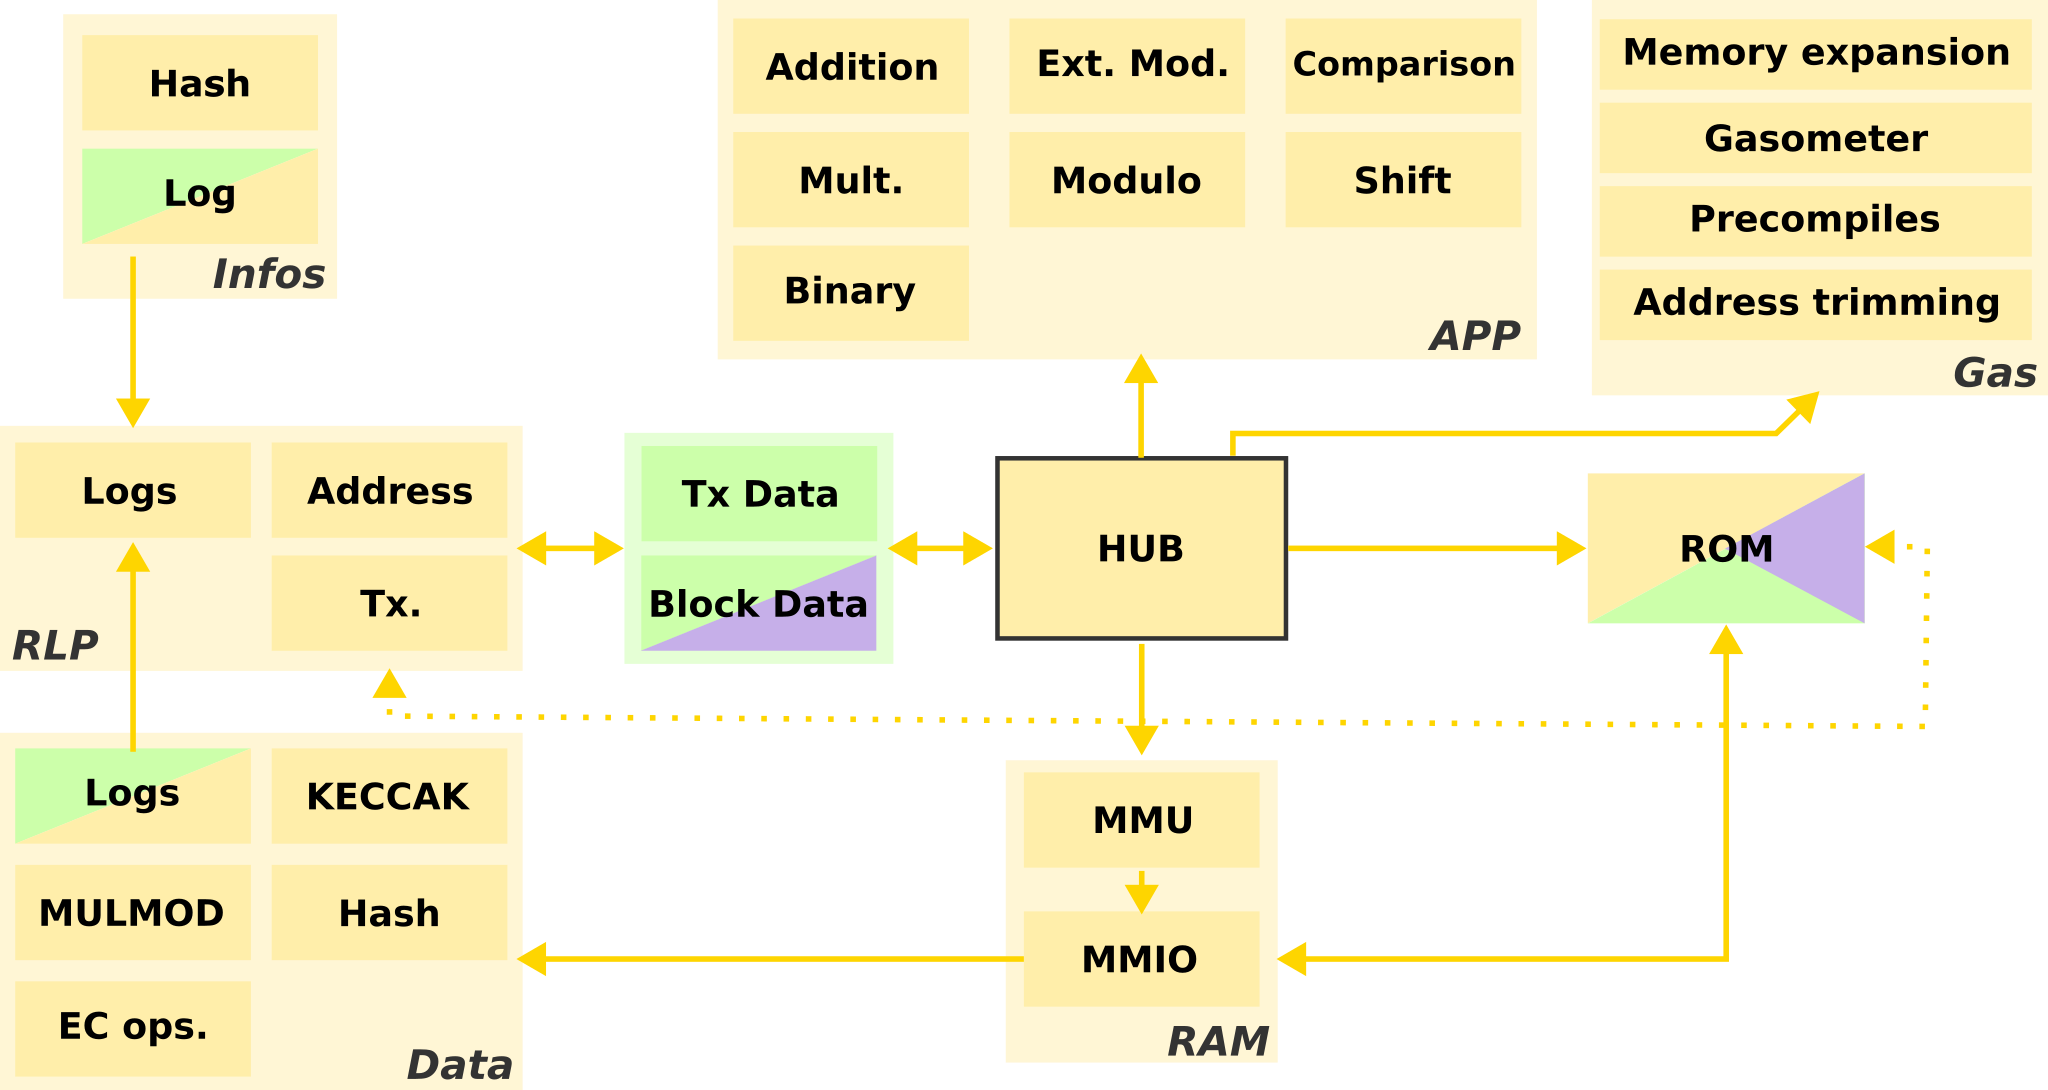
\includegraphics[width = \textwidth]{../img/zkevm_better_arrow_heads.png}
\caption{Modular architecture of the zk-evm. Boxes represent modules and arrows represent lookup inclusions. If an arrow points from module \col{ABC} to module \col{XYZ} then \col{XYZ} imports a portion of its data from \col{ABC}.  Arrows may be bidirectional which signals a ``bilateral'' inclusion proof.}
\end{figure}
